\clearpage
\section{Работа с моделями в GPSS World}
\label{sec:evidence}

\subsection{Двухприборная СМО}

На рисунках~\ref{fig:gp-system-model}–\ref{fig:gp-system-report}
показаны последовательные шаги контрольного опыта системы 33.
После трансляции выполнен прогрев на \(10\,000\) исходов. Затем
команда \texttt{RESET} сбросила статистику, и команда
\texttt{START 120000} запустила измерительный прогон.

\begin{figure}[H]
 \centering
 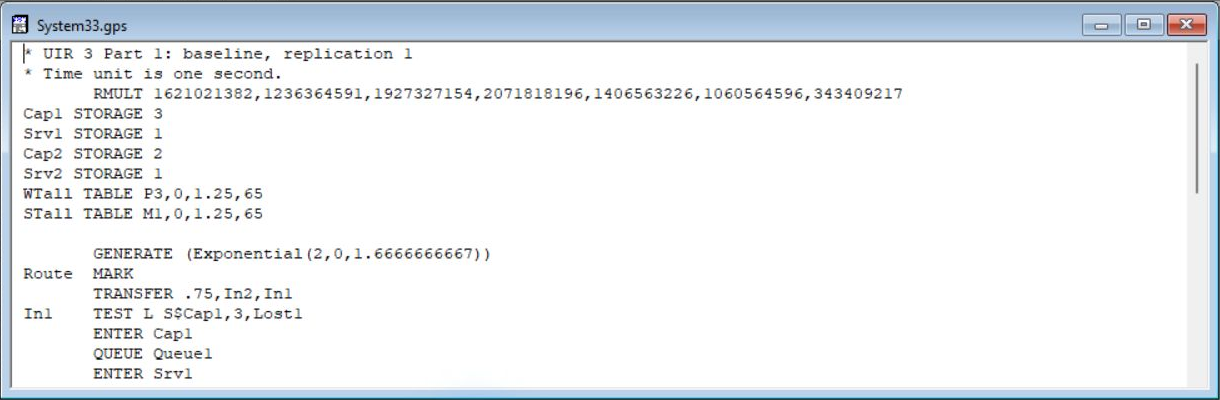
\includegraphics[width=.96\textwidth]{evidence/01_model_system33.png}
 \caption{Исходная модель системы 33 в редакторе GPSS World.
 Первая ветвь вмещает три заявки всего, вторая — две}
 \label{fig:gp-system-model}
\end{figure}

\begin{figure}[H]
 \centering
 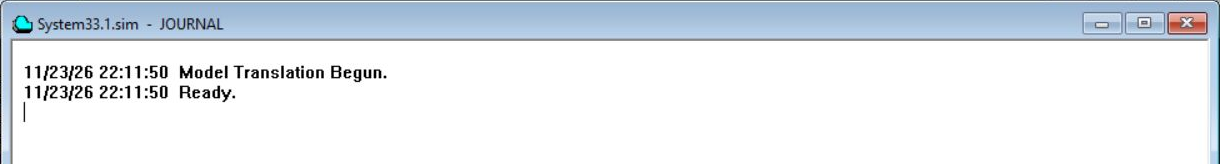
\includegraphics[width=.96\textwidth]{evidence/02_translation_system33.png}
 \caption{Журнал трансляции модели. Сообщение \texttt{Ready} подтверждает
 готовность имитационной модели к запуску}
 \label{fig:gp-system-translation}
\end{figure}

\begin{figure}[H]
 \centering
 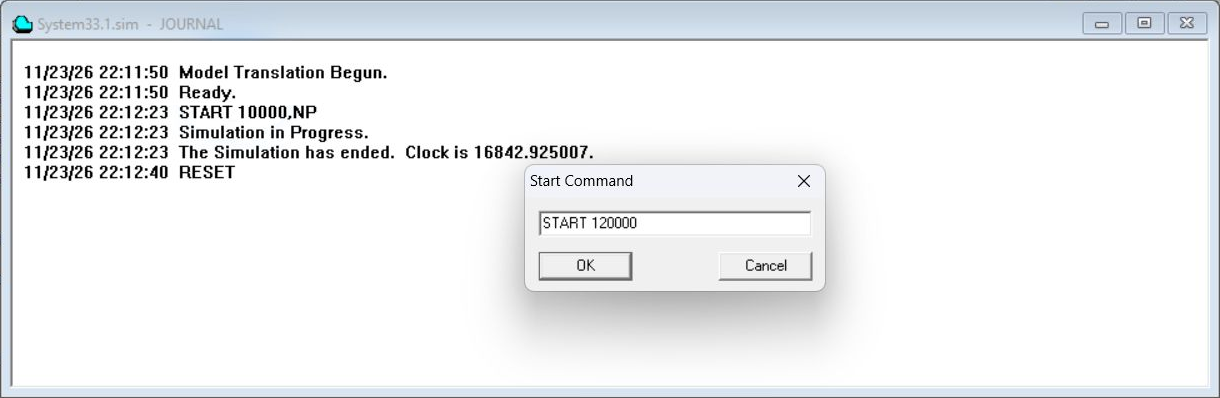
\includegraphics[width=.96\textwidth]{evidence/03_start_system33.png}
 \caption{Настройка измерительного прогона. Журнал показывает выполненный
 прогрев и сброс статистики, в диалоге задана команда \texttt{START 120000}}
 \label{fig:gp-system-start}
\end{figure}

\begin{figure}[H]
 \centering
 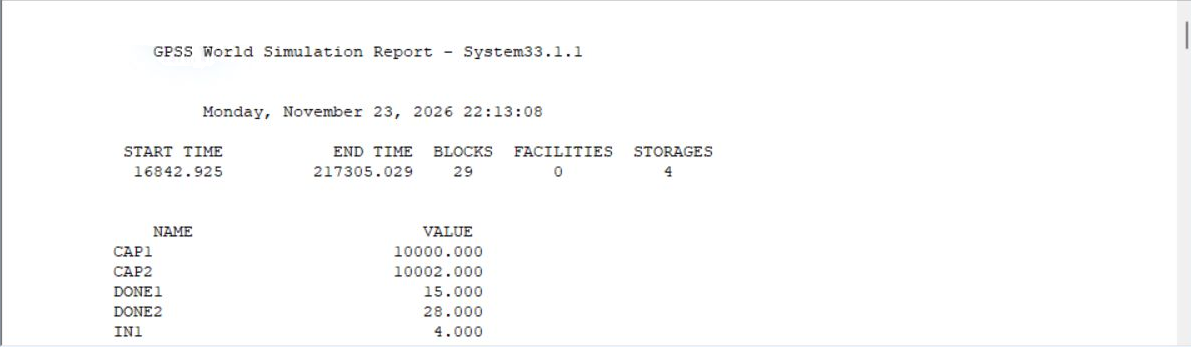
\includegraphics[width=.96\textwidth]{evidence/04_report_system33.png}
 \caption{Стандартный отчёт системы 33. Измерительный интервал
 \(16\,842{,}925\)–\(217\,305{,}029\) с}
 \label{fig:gp-system-report}
\end{figure}

\subsection{Замкнутая сеть M3}

На рисунке~\ref{fig:gp-network-model} открыта контрольная модель
с шестью циркулирующими заявками, а на рисунке~\ref{fig:gp-network-report}
виден отчёт прогона после \(10\,000\) с прогрева.
Статистика собрана за \(200\,000\) с модельного времени.

\begin{figure}[H]
 \centering
 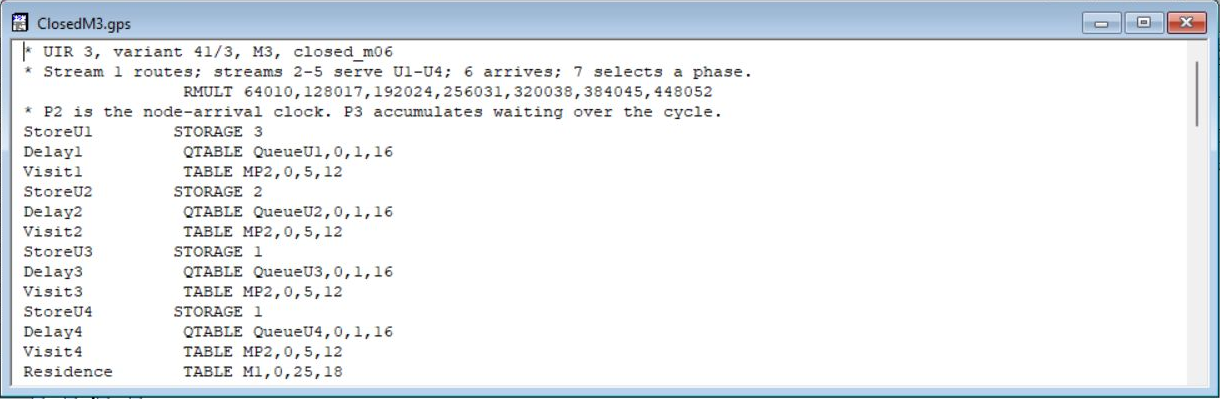
\includegraphics[width=.96\textwidth]{evidence/05_model_network.png}
 \caption{Модель замкнутой сети M3 в редакторе GPSS World.
 Параметры четырёх узлов заданы командами \texttt{STORAGE}}
 \label{fig:gp-network-model}
\end{figure}

\begin{figure}[H]
 \centering
 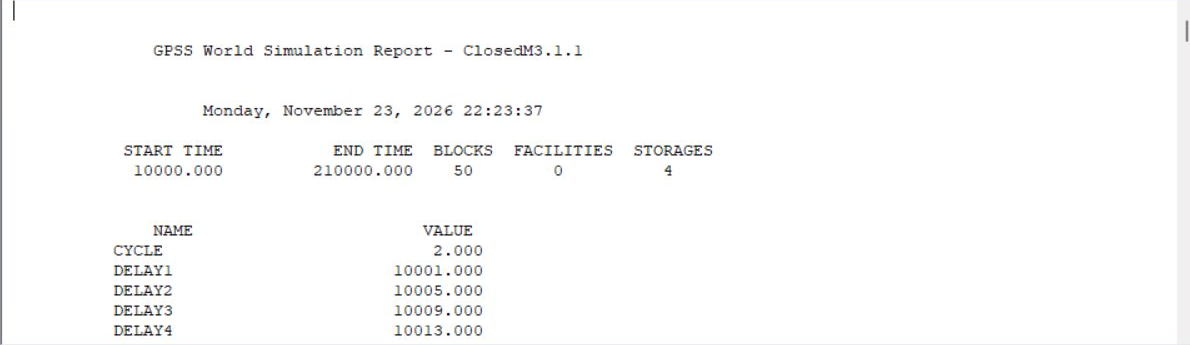
\includegraphics[width=.96\textwidth]{evidence/06_report_network.png}
 \caption{Стандартный отчёт контрольного прогона замкнутой сети при \(M=6\)}
 \label{fig:gp-network-report}
\end{figure}

\clearpage
\subsection{Серия парных прогонов сети M3}

На рисунке~\ref{fig:gp-network-campaign} показан журнал эксперимента,
который сравнивает замкнутую и разомкнутую сети при сопоставимой
интенсивности. Записи с отметками \(100\,000\) и \(900\,000\) с
соответствуют концу прогрева и измерения. Процедура PLUS сохраняет
сводку после каждого измерения в CSV.

\begin{figure}[H]
 \centering
 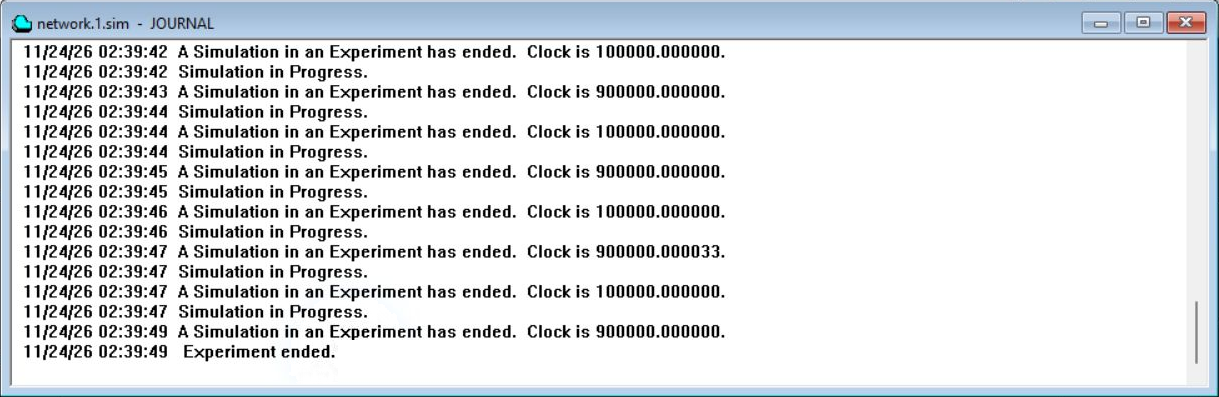
\includegraphics[width=.96\textwidth]{evidence/07_campaign_network.png}
 \caption{Журнал \texttt{network.1.sim} после завершения серии парных прогонов}
 \label{fig:gp-network-campaign}
\end{figure}
